\chapter{约束满足问题}

\section{约束满足问题}

\subsection{约束满足问题(CSP, Constraint Satisfaction Problems)}

在CSP问题中,存在一组变量,当每个变量都被赋了一个值,且能够满足所有的约束条件时,问题就解决了。\\

CSP问题包含:

\begin{itemize}
    \item $ X = \{X_1, X_2, \cdots, X_n\} $:变量集合
    \item $ D = \{D_1, D_2, \cdots, D_n\} $:域(domain)
    \item $ C $:约束集合
\end{itemize}

约束可分为:

\begin{itemize}
    \item 一元约束(unary constraint):只对一个变量进行约束,如$ A \neq 3 $、$ B \neq 4 $。
    \item 二元约束(binary constraint):对两个变量进行约束,如$ A < B $、$ B < C $。
    \item 多元约束:对两个以上的变量进行约束,如$ A + B < C $。
\end{itemize}

例如$ X = \{A, B, C\} $,$ dom(A) = dom(B) = dom(C) = \{1, 2, 3, 4\} $,约束条件为$ A < B $和$ B < C $。\\

其中$ A = 2 $、$ B = 3 $、$ C = 4 $是一组满足要求的赋值,而$ A = 2 $、$ B = 3 $、$ C = 1 $就是一组不满足要求的赋值。\\

\subsection{澳大利亚地图着色问题}

在澳大利亚地图着色问题中,

\begin{itemize}
    \item $ X = \{WA, NT, SA, Q, NSW, V, T\} $
    \item $ D = \{Red, Green, Blue\} $
    \item $ C = \{SA \neq WA, SA \neq NT, SA \neq Q, SA \neq V, SA \neq NSW, WA \neq NT, NT \neq Q, Q \neq NSW, NSW \neq V\} $
\end{itemize}

\begin{figure}[H]
    \centering
    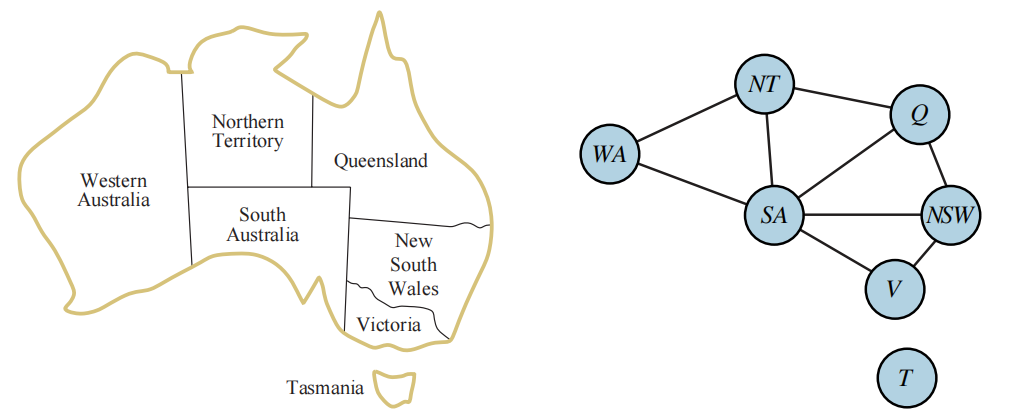
\includegraphics[scale=0.45]{img/C2/2-1/1.png}
    \caption{澳大利亚地图}
\end{figure}

\vspace{0.5cm}

\subsection{密码算术谜题}

在密码算术谜题中,每个字母代表一个不同的数字。

\begin{table}[H]
    \centering
    \begin{tabular}{cD{.}{.}{3}}
          & TWO  \\
        + & TWO  \\
        \hline
        = & FOUR
    \end{tabular}
\end{table}

\begin{itemize}
    \item 变量
          \begin{itemize}
              \item $ X = \{T, W, O, F, U, R, C_1, C_2, C_3\} $,其中$ C_1 $、$ C_2 $、$ C_3 $为进位。
          \end{itemize}
    \item 域
          \begin{itemize}
              \item $ dom(T) = dom(W) = dom(O) = dom(F) = dom(U) = dom(R) = \{0, 1, \cdots, 9\} $
              \item $ dom(C_1) = dom(C_2) = dom(C_3) = \{0, 1\} $
          \end{itemize}
    \item 约束
          \begin{itemize}
              \item $ AllDiff(T, W, O, F, U, R)  $
              \item $ O + O = R = 10C_1 $
              \item $ C_1 + W + W = U + 10C_2 $
              \item $ C_2 + T + T = O + 10C_3 $
              \item $ C_3 = F $
              \item $ T \neq 0 $
              \item $ F \neq 0 $
          \end{itemize}
\end{itemize}

\vspace{0.5cm}

\subsection{数独}

数独的目标是在$ 9 \times 9 $的方格中填入数字,使得每一行、每一列和每一个$ 3 \times 3 $的小方格中都包含$ 1 \sim 9 $的数字。\\

\begin{sudoku}
    | | |3| |2| |6| | |.
    |9| | |3| |5| | |1|.
    | | |1|8| |6|4| | |.
    | | |8|1| |2|9| | |.
    |7| | | | | | | |8|.
    | | |6|7| |8|2| | |.
    | | |2|6| |9|5| | |.
    |8| | |2| |3| | |9|.
    | | |5| |1| |3| | |.
\end{sudoku}

假设数独的行号为$ A \sim I $,列号为$ 1 \sim 9 $。

\begin{itemize}
    \item 变量
          \begin{itemize}
              \item $ X = \{A1, \cdots, A9, B1, \cdots \cdots, I1, \cdots I9\} $
          \end{itemize}
    \item 域
          \begin{itemize}
              \item $ D = \{1, 2, 3, 4, 5, 6, 7, 8, 9\} $
          \end{itemize}
    \item 约束
          \begin{itemize}
              \item $ AllDiff(A1, A2, A3, A4, A5, A6, A7, A8, A9) $
              \item $ AllDiff(B1, B2, B3, B4, B5, B6, B7, B8, B9) $
              \item $ \cdots $
              \item $ AllDiff(A1, B1, C1, D1, E1, F1, G1, H1, I1) $
              \item $ AllDiff(A2, B2, C2, D2, E2, F2, G2, H2, I2) $
              \item $ \cdots $
              \item $ AllDiff(A1, A2, A3, B1, B2, B3, C1, C2, C3) $
              \item $ AllDiff(A4, A5, A6, B4, B5, B6, C4, C5, C6) $
              \item $ \cdots $
          \end{itemize}
\end{itemize}

\newpage

\section{约束传播}

\subsection{约束传播(Constrain Propagation)}

